%% Please do not use \input{...} to include other tex files.
%% Submit your LaTeX manuscript as one .tex document.
%%
%% All additional figures and files should be attached
%% separately and not embedded in the \TeX\ document itself.
%%
%%%%%%%%%%%%%%%%%%%%%%%%%%%%%%%%%%%%%%%%%%%%%%%%%%%%%%%%%%%%%%%%%%%%%

%%\documentclass[referee,sn-basic]{sn-jnl}% referee option is meant for double line spacing

%%=======================================================%%
%% to print line numbers in the margin use lineno option %%
%%=======================================================%%

%%\documentclass[lineno,pdflatex,sn-basic]{sn-jnl}% Basic Springer Nature Reference Style/Chemistry Reference Style

%%=========================================================================================%%
%% the documentclass is set to pdflatex as default. You can delete it if not appropriate.  %%
%%=========================================================================================%%

%%\documentclass[sn-basic]{sn-jnl}% Basic Springer Nature Reference Style/Chemistry Reference Style

%%Note: the following reference styles support Namedate and Numbered referencing. By default the style follows the most common style. To switch between the options you can add or remove “Numbered” in the optional parenthesis. 
%%The option is available for: sn-basic.bst, sn-chicago.bst%  
 
%%\documentclass[pdflatex,sn-nature]{sn-jnl}% Style for submissions to Nature Portfolio journals
%%\documentclass[pdflatex,sn-basic]{sn-jnl}% Basic Springer Nature Reference Style/Chemistry Reference Style
\documentclass[pdflatex,sn-mathphys-num]{sn-jnl}% Math and Physical Sciences Numbered Reference Style
%%\documentclass[pdflatex,sn-mathphys-ay]{sn-jnl}% Math and Physical Sciences Author Year Reference Style
%%\documentclass[pdflatex,sn-aps]{sn-jnl}% American Physical Society (APS) Reference Style
%%\documentclass[pdflatex,sn-vancouver-num]{sn-jnl}% Vancouver Numbered Reference Style
%%\documentclass[pdflatex,sn-vancouver-ay]{sn-jnl}% Vancouver Author Year Reference Style
%%\documentclass[pdflatex,sn-apa]{sn-jnl}% APA Reference Style
%%\documentclass[pdflatex,sn-chicago]{sn-jnl}% Chicago-based Humanities Reference Style
% \usepackage[a4paper, total={6.5in, 9in}]{geometry}
%%%% Standard Packages
%%<additional latex packages if required can be included here>

\usepackage{graphicx}%
\usepackage{multirow}%
\usepackage{amsmath,amssymb,amsfonts}%
\usepackage{amsthm}%
\usepackage{mathrsfs}%
\usepackage[title]{appendix}%
\usepackage{xcolor}%
\usepackage{textcomp}%
\usepackage{manyfoot}%
\usepackage{booktabs}%
\usepackage{algorithm}%
\usepackage{algorithmicx}%
\usepackage{algpseudocode}%
\usepackage{listings}%
%%%%

%%%%%=============================================================================%%%%
%%%%  Remarks: This template is provided to aid authors with the preparation
%%%%  of original research articles intended for submission to journals published 
%%%%  by Springer Nature. The guidance has been prepared in partnership with 
%%%%  production teams to conform to Springer Nature technical requirements. 
%%%%  Editorial and presentation requirements differ among journal portfolios and 
%%%%  research disciplines. You may find sections in this template are irrelevant 
%%%%  to your work and are empowered to omit any such section if allowed by the 
%%%%  journal you intend to submit to. The submission guidelines and policies 
%%%%  of the journal take precedence. A detailed User Manual is available in the 
%%%%  template package for technical guidance.
%%%%%=============================================================================%%%%

%% as per the requirement new theorem styles can be included as shown below
\theoremstyle{thmstyleone}%
\newtheorem{theorem}{Theorem}%  meant for continuous numbers
%%\newtheorem{theorem}{Theorem}[section]% meant for sectionwise numbers
%% optional argument [theorem] produces theorem numbering sequence instead of independent numbers for Proposition
\newtheorem{proposition}[theorem]{Proposition}% 
%%\newtheorem{proposition}{Proposition}% to get separate numbers for theorem and proposition etc.

\theoremstyle{thmstyletwo}%
\newtheorem{example}{Example}%
\newtheorem{remark}{Remark}%

\theoremstyle{thmstylethree}%
\newtheorem{definition}{Definition}%

\raggedbottom
%%\unnumbered% uncomment this for unnumbered level heads
%% Reduce footnote spacing
\setlength{\skip\footins}{5pt}  % reduces space between main text and footnote
\renewcommand{\footnotesize}{\fontsize{8}{9}\selectfont} % smaller font and line spacing

\begin{document}

\title[RL for Pseudo-Labeling]{Reinforcement Learning for Pseudo-Labeling}

%%=============================================================%%
%% GivenName    -> \fnm{Joergen W.}
%% Particle -> \spfx{van der} -> surname prefix
%% FamilyName   -> \sur{Ploeg}
%% Suffix   -> \sfx{IV}
%% \author*[1,2]{\fnm{Joergen W.} \spfx{van der} \sur{Ploeg} 
%%  \sfx{IV}}\email{iauthor@gmail.com}
%%=============================================================%%

\author[1]{\fnm{Aishwarya} \sur{Maddula}}
\author[1]{\fnm{Deepika} \sur{Reddygari}}
\author*[1]{\fnm{Phanindra} \sur{Kalaga}}\email{phanindra.connect@gmail.com}
\author[1]{\fnm{Prudhvi} \sur{Chekuri}}

\affil*[1]{\orgdiv{Data Science}, \orgname{The George Washington University}, \orgaddress{\city{Washington}, \state{DC}, \country{USA}}}

%%==================================%%
%% Sample for unstructured abstract %%
%%==================================%%

\abstract{Semi-supervised learning leverages abundant unlabeled data to improve performance when labeled data is scarce. This work develops a reinforcement learning (RL) framework for intelligent pseudo-labeling, where an RL agent learns to assign high-quality pseudo-labels to unlabeled samples. We implement and evaluate both a Policy Gradient approach using a custom OpenAI Gymnasium environment and a Reinforcement Learning-Guided Semi-Supervised Learning (RLGSSL) framework with teacher-student learning and mixup augmentation. Our framework formulates pseudo-labeling as a sequential decision-making problem, with state representations based on CNN features, model predictions, and prediction entropy. Experimental results demonstrate substantial improvements: achieving 3.45\% error rate on MNIST with a CNN (from 54\% baseline) and 25.75\% error rate on CIFAR-10 with ResNet-18 (from 34.40\% baseline). We identify key challenges including reward function design, computational complexity, and training stability that provide valuable insights for future work in RL-guided semi-supervised learning.}

\keywords{Semi-Supervised Learning, Reinforcement Learning, Pseudo-Labeling, RLGSSL}

%%\pacs[JEL Classification]{D8, H51}

%%\pacs[MSC Classification]{35A01, 65L10, 65L12, 65L20, 65L70}

\maketitle

\section{Introduction}\label{sec1}

In modern machine learning applications, obtaining large quantities of labeled training data is often expensive, time-consuming, and requires domain expertise. Semi-supervised learning (SSL) offers a promising solution by leveraging both limited labeled data and abundant unlabeled data to improve model performance. A key technique in SSL is pseudo-labeling, where a model assigns estimated labels to unlabeled samples, which are then used for further training.

Traditional pseudo-labeling approaches rely on simple heuristics such as confidence thresholds, often selecting pseudo-labels based solely on prediction confidence. However, these methods can propagate errors when incorrect high-confidence predictions are blindly accepted, leading to confirmation bias \cite{arazo2020pseudolabelingconfirmationbiasdeep} and degraded model performance.

This work addresses these limitations by framing pseudo-labeling as a reinforcement learning problem. By treating the selection and assignment of pseudo-labels as a sequential decision-making task, we enable an intelligent agent to learn optimal labeling strategies that balance exploration (diverse samples) and exploitation (high-confidence samples).

We explore two complementary approaches to RL-based pseudo-labeling:
\begin{enumerate}
    \item \textbf{Custom RL Environment with Policy Gradients}: A complete RL framework implemented from scratch, including a custom \texttt{PseudoLabelEnv} environment implementing the OpenAI Gymnasium interface, state representations capturing image features and model uncertainty, and confidence-driven reward structures.
    \item \textbf{RLGSSL Framework}: An implementation of the Reinforcement Learning-Guided Semi-Supervised Learning approach proposed by Heidari et al.~\cite{heidari2024rlgssl}, which integrates a Teacher-Student framework utilizing Exponential Moving Average (EMA) for stable target generation, mixup data augmentation for continuous training signals, and adaptive enhancements to improve stability and diversity.
\end{enumerate}

\section{Literature Review}\label{sec:lit_review}

Semi-supervised learning has been extensively studied as a paradigm for learning from limited labeled data. Key approaches include Consistency Regularization (e.g., MixMatch, FixMatch), Self-Training, and Graph-Based Methods. Unlike these methods which often use fixed heuristics for pseudo-label selection, our RL-based approach learns adaptive selection strategies.

Traditional pseudo-labeling assigns labels to unlabeled samples based on model predictions exceeding a confidence threshold. Recent improvements include Confidence-Based Selection \cite{sohn2020fixmatchsimplifyingsemisupervisedlearning}, Temporal Ensembling (Mean Teacher), and MixUp Augmentation. RL has also been explored for selective pseudo-labeling in domain adaptation contexts \cite{liu2020selectivepseudolabelingreinforcementlearning}.

Our primary inspiration comes from Heidari et al. \cite{heidari2024rlgssl}, who proposed RLGSSL, a framework that formulates semi-supervised learning as a reinforcement learning problem. Their key contributions include using the classification network itself as the RL policy, implementing reward signals derived from model performance on synthetically mixed samples (Mixup), and a novel loss formulation based on KL divergence weighting:
\\
\begin{equation}
\mathcal{L}_{rl} = -\mathbb{E}_{y_i^u \sim \pi_\theta} [\text{KL}(e, y_i^u) \times R(s,a;\text{sg}[\theta])]
\end{equation}
\\
Our work differs by exploring both custom RL environments with explicit state-action formulations and integrated RLGSSL approaches. We also introduce adaptive enhancements including confidence bonuses, diversity regularization, and curriculum learning mechanisms.

\section{Methodology}\label{sec:method}

We developed a comprehensive approach to RL-based pseudo-labeling, hypothesizing that a learnable policy can outperform static thresholds by adapting to the changing reliability of the downstream classifier during training. To test this, we designed two distinct implementations. The first is a modular architecture using a custom OpenAI Gymnasium environment, and the second is an integrated RLGSSL-based approach where the classifier and policy are unified.

\subsection{Gymnasium}\label{subsec:gym}

To formalize the interaction between the labeling agent and the unlabeled dataset, we implemented a custom OpenAI Gymnasium environment, \texttt{PseudoLabelEnv}. This environment serves as a wrapper, abstracting the complexities of data loading and feature extraction into a standard RL interface. The overall system flow is illustrated in Figure \ref{fig:system_flow}.

\begin{figure}[h]
\centering
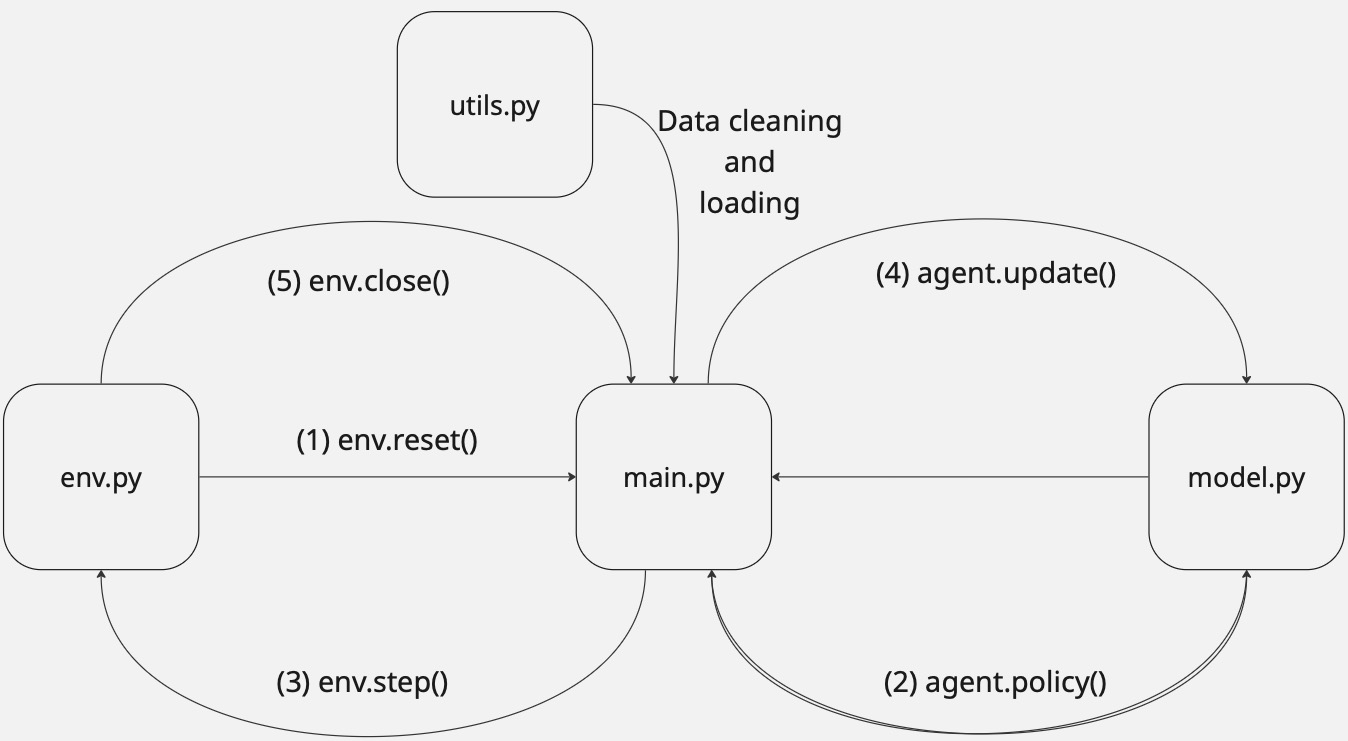
\includegraphics[width=0.95\linewidth]{Fig/flowchart.jpeg}
\caption{Architecture of the custom RL pseudo-labeling environment, showing interactions between the environment, agent, and downstream model.}
\label{fig:system_flow}
\end{figure}

The environment manages the lifecycle of the training process through standard methods:
\begin{itemize}
    \item \textbf{Initialization (\texttt{reset})}: At the start of an episode, the environment resets internal counters and prepares the first batch of unlabeled samples. Depending on the specific experimental configuration, the downstream model may be re-initialized to prevent overfitting or preserved to simulate continuous learning.
    \item \textbf{Transition (\texttt{step})}: This method executes the core logic of the MDP. Upon receiving an action for the current sample $x_i$, the environment evaluates the correctness of the action (internally using ground truth during training phases), computes the reward $r_i$, and constructs the subsequent state $s_{i+1}$. It returns this tuple along with a termination flag.
\end{itemize}

The training loop for the RL agent follows the procedure outlined in Algorithm \ref{alg:rl_training}.

\begin{algorithm}[h]
\caption{RL agent training loop}
\label{alg:rl_training}
\scriptsize
\begin{algorithmic}[1]
  \Require state\_dim, action\_dim, labeled\_data, unlabeled\_data, num\_episodes
  \State agent $\leftarrow$ \texttt{RLAgent}(state\_dim, action\_dim)
  \State env $\leftarrow$ \texttt{PseudoLabelEnv}(labeled\_data, unlabeled\_data)
  \For{episode = 1 \textbf{to} num\_episodes}
  \State state $\leftarrow$ env.reset()
  \State done $\leftarrow$ false
  \While{not done}
  \State action $\leftarrow$ agent.select\_action(state)
  \State $(\text{next\_state},\ \text{reward},\ \text{terminated},\ \text{info}) \leftarrow \text{env.step(action)}$
  \State state $\leftarrow$ next\_state
  \State done $\leftarrow$ terminated
  \EndWhile
  \State agent.update()
  \State accuracy $\leftarrow$ env.evaluate()
  \EndFor
  \State env.close()
\end{algorithmic}
\end{algorithm}

\subsection{MDP Formulation}\label{subsec:mdp}

We formulate the problem as a Markov Decision Process (MDP), which mathematically models the sequential decision-making required to label a stream of data points. The components of the MDP are defined as follows:

\begin{itemize}

    \item \textbf{State Space ($\mathcal{S}$)}: The state representation is crucial for the agent to gauge the reliability of the downstream model. For each unlabeled sample $x_i$, the state $s_i$ is constructed as a concatenation of three distinct feature sets:
    \begin{equation}
     s_i = [\phi(x_i), P_\theta(x_i), H(P_\theta(x_i))]
    \end{equation}
    Here, $\phi(x_i)$ represents the flattened high-level image features extracted by the CNN, providing semantic context. $P_\theta(x_i)$ denotes the softmax class probabilities, representing the model's current belief distribution. Finally, $H(P_\theta(x_i))$ is the prediction entropy, serving as a scalar measure of epistemic uncertainty.
    
    \item \textbf{Action Space ($\mathcal{A}$)}: The action space defines the choices available to the agent. For a classification problem with $K$ classes, we define a discrete action space:
    \begin{equation}
    \mathcal{A} = \{0, 1, \ldots, K-1, \text{skip}\}.
    \end{equation}
    Actions $0$ through $K-1$ correspond to assigning a specific pseudo-label to the sample $x_i$. Crucially, we introduce a $\text{skip}$ action. This allows the agent to act conservatively, opting not to label a sample if the confidence is low or the state is ambiguous, thereby preventing the contamination of the training set with noisy labels.
    
    \item \textbf{Reward Function ($R$)}: The reward function drives the policy optimization. We utilize two distinct reward structures depending on the framework:
    \begin{enumerate}
        \item \textit{Custom Environment (Training)}: When ground truth $y_i^{\text{true}}$ is accessible for the reward signal (but hidden from the input), we use a confidence-weighted reward:
        \begin{equation}
        R(s_i, a_i) = \begin{cases}
        -0.1 & \text{if } a_i = \text{skip} \\
        P_\theta(x_i)_{a_i} & \text{if } a_i = y_i^{\text{true}} \\
        -P_\theta(x_i)_{a_i} & \text{if } a_i \neq y_i^{\text{true}}
        \end{cases}
        \end{equation}
        This penalizes incorrect high-confidence guesses heavily while applying a small penalty for skipping to encourage eventual labeling.
        
        \item \textit{RLGSSL}: In the absence of ground truth, the reward is derived from consistency. We measure the Mean Squared Error (MSE) between predictions on original and Mixup-augmented samples:
        \begin{equation}
        R(s, a; \text{sg}[\theta]) = -\text{MSE}(P_\theta(x_i^m), y_i^m)
        \end{equation}
        This reward encourages the model to be invariant to perturbations, a core tenet of semi-supervised learning.
    \end{enumerate}
    
    \item \textbf{Terminal State}: An episode is defined as one complete pass through the available batch of unlabeled data. The terminal state is reached when all $N$ samples in the current buffer have been processed (either labeled or skipped).
\end{itemize}

\subsection{Models}\label{subsec:models}

\subsubsection{Downstream Model}
The downstream model acts as the primary classifier for the task and, in our architecture. For our experiments on the MNIST dataset, we constructed a Convolutional Neural Network (CNN). The architecture consists of two 2D convolutional layers with ReLU activation to extract spatial hierarchies, followed by max-pooling layers for dimensionality reduction. The output is flattened and passed through fully connected dense layers to produce the logits:
\begin{equation}
\text{logits} = \text{CNN}(x; \theta)
\end{equation}
These logits are converted to probabilities via Softmax to form the prediction component of the RL state.

\subsubsection{RL Agents}
We investigated two distinct agent architectures to solve the MDP:

\textbf{Policy Gradient Agent}: This agent utilizes an Actor-Critic architecture explicitly separated from the classifier. The \textit{Actor} network takes the state $s_i$ and outputs a probability distribution over the action space $\mathcal{A}$. The \textit{Critic} network estimates the value function $V(s_i)$ to reduce the variance of the gradient updates. This separation allows for precise control over the labeling policy but requires training two distinct sets of parameters.

\textbf{RLGSSL Agent}: In this integrated approach, the classification network itself functions as the RL policy $\pi_\theta$. The network parameters $\theta$ are optimized to simultaneously minimize the supervised classification loss on labeled data and maximize the expected reward on unlabeled data. The RL objective is formulated as:
\begin{equation}
\mathcal{L}_{\text{rl}} = -\mathbb{E}_{y_i^u \sim \pi_\theta} [\text{KL}(e, y_i^u) \times R(s,a;\text{sg}[\theta])]
\end{equation}
Here, the Kullback-Leibler (KL) divergence term acts as a weighting mechanism, and the reward signal directs the gradient updates. To improve stability, we integrated adaptive enhancements, including confidence bonuses and diversity regularization, to prevent the policy from collapsing into a trivial solution (e.g., predicting a single class).

\subsection{Metrics}\label{subsec:metrics}
To rigorously evaluate the performance of our RL frameworks, we tracked the following metrics:

\begin{itemize}
    \item \textbf{Accuracy}: The primary measure of utility, calculated as the ratio of correct predictions to total predictions on the held-out validation set:
    \begin{equation}
        \text{Accuracy} = \frac{1}{N_{val}} \sum_{i=1}^{N_{val}} \mathbb{I}(\hat{y}_i = y_i)
    \end{equation}
    \item \textbf{RL Loss}: This metric tracks the convergence of the policy optimization. For the Policy Gradient agent, it represents the combined actor and critic losses. For RLGSSL, it is the specific component $\mathcal{L}_{\text{rl}}$ responsible for pseudo-label optimization.
    \item \textbf{Average Reward}: This serves as a proxy for the quality of the pseudo-labels generated during training. It is calculated per episode or batch as:
    \begin{equation}
        \bar{R} = \frac{1}{T} \sum_{t=1}^{T} r_t
    \end{equation}
    A rising average reward indicates that the agent is learning to select correct labels with higher confidence.
\end{itemize}

\section{Results}\label{sec:results}

\subsection{Policy Gradient Results}
The Policy Gradient agent demonstrated adaptive behavior, learning to balance pseudo-labeling and selective skipping based on model confidence. We evaluated the approach across multiple datasets and architectures. Table \ref{tab:pg_results} summarizes the key results.

\begin{table}[h]
\caption{Policy Gradient error rates across datasets and architectures.}\label{tab:pg_results}
\begin{tabular}{@{}llcc@{}}
\toprule
Dataset & Model & Error Rate \\
\midrule
MNIST & CNN & \textbf{3.45\%} \\
MNIST & MLP & 37.40\% \\
MNIST & ResNet-18 & 5.80\% \\
CIFAR-10 & CNN & 34.40\% \\
CIFAR-10 & MLP & 59.60\% \\
CIFAR-10 & ResNet-18 & \textbf{25.75\%} \\
\bottomrule
\end{tabular}
\end{table}

On MNIST with 18,000 labeled samples and 40,000 unlabeled samples, the Policy Gradient agent achieved a best error rate of 3.45\% with the CNN architecture, representing a substantial improvement from an initial baseline error rate of approximately 54\%. The MLP architecture showed higher error rates (37.40\%), while ResNet-18 achieved 5.80\% error rate.

For CIFAR-10, the ResNet-18 architecture achieved the best performance with a 25.75\% error rate, demonstrating that stronger pretrained features provide more stable improvements. The CNN architecture achieved 34.40\% error rate, while MLP showed higher error rates of 59.60\%.

\subsection{RLGSSL Results}
Table \ref{tab:rlgssl_training} shows the training progression on CIFAR-10 with 1000 labeled samples using the RLGSSL framework.

\begin{table}[h]
\caption{RLGSSL training progression on CIFAR-10 (1000 labels).}\label{tab:rlgssl_training}
\begin{tabular}{@{}lllll@{}}
\toprule
Epoch & Error (\%) & Loss & RL Loss & Reward \\
\midrule
50 (warmup) & 53.61 & 0.137 & -0.00533 & -0.0305 \\
100 & 74.02 & 0.233 & 0.018 & -0.0298 \\
150 & 66.56 & 0.215 & 0.013 & -0.0290 \\
250 & 59.48 & 0.188 & 0.005 & -0.0290 \\
350 & 61.51 & 0.160 & -0.00464 & -0.0283 \\
450 & \textbf{58.59} & 0.133 & -0.03042 & -0.0282 \\
\bottomrule
\end{tabular}
\end{table}

The RLGSSL framework achieved a best error rate of 53.8\% after approximately 10 hours of training on CIFAR-10 with 1000 labeled samples. The RL reward signal showed consistent improvement throughout training, trending from approximately $-0.0305$ to $-0.0282$ over 450 epochs, indicating that the agent learned to make increasingly better pseudo-labeling decisions. We observed initial instability when RL loss was introduced after warmup (error increased to 74.02\% at epoch 100), followed by gradual recovery and stabilization.

\textbf{Comparison with Literature:} Our best observed error rate of 53.8\% is significantly higher than the paper's reported 9.15\% error. This discrepancy likely stems from potential implementation differences in adaptive enhancements, the need for more careful hyperparameter tuning, and possible differences in data preprocessing or augmentation strategies.

\subsection{Key Observations}

Both RL-based approaches demonstrated the feasibility of intelligent pseudo-labeling:
\begin{itemize}
    \item \textbf{Policy Gradient}: Achieved best error rates of 3.45\% on MNIST (CNN) and 25.75\% on CIFAR-10 (ResNet-18), representing substantial improvements from initial baseline error rates of approximately 54\%.
    \item \textbf{RLGSSL}: Showed stable training dynamics with consistent reward improvement, though a significant performance gap remained compared to state-of-the-art benchmarks.
\end{itemize}

\section{Discussion}\label{sec:discussion}

The application of Reinforcement Learning to the task of pseudo-labeling presents a complex set of trade-offs between adaptability and stability. Our experiments revealed several important insights that differentiate this approach from static heuristic methods.

\textbf{Overview of Findings}: The Policy Gradient agent demonstrated adaptive behavior, successfully learning to balance pseudo-labeling with skipping uncertain samples. The RLGSSL framework showed promise with stable training dynamics. Despite successfully implementing full pipelines, we observed significant performance gaps compared to state-of-the-art benchmarks, primarily driven by computational constraints preventing full convergence and numerical instabilities in adaptive reward enhancements.

\textbf{Reward Function Design}: Designing effective reward functions proved to be one of the most challenging aspects. Sparse vs.\ dense rewards presented an issue: initial experiments with only end-of-episode error rate rewards provided insufficient learning signal, while adding per-step confidence-based rewards improved learning but introduced new challenges. Reward scaling was difficult, as balancing the magnitude of step rewards (confidence values in [0,1]) with episode-end error rate bonuses required careful tuning. Stability issues emerged because adaptive reward enhancements in RLGSSL introduced numerical instability; the diversity bonus, in particular, may have caused gradient explosions when batch entropy varied significantly.

\textbf{Computational Constraints}: The computational demands of RL-based pseudo-labeling present significant practical barriers. Episode length was a concern because each Policy Gradient episode processes thousands of unlabeled samples, resulting in lengthy episodes and delayed learning. Training times exceeded 10+ hours, highlighting the need for GPU acceleration. Memory requirements also posed challenges, as maintaining teacher and student models simultaneously doubles memory requirements compared to standard training.

\textbf{Non-Stationarity and Credit Assignment}: The pseudo-labeling environment violates key RL assumptions. The moving target issue arises because the downstream model evolves during training, causing state distributions to shift continuously and challenging standard RL convergence guarantees. Delayed feedback complicates training because error rate improvements may not manifest until many episodes later, making credit assignment difficult.

\textbf{Insights on RLGSSL Formulation}: Through implementation, we gained several insights. The elegant formulation where the classifier itself serves as the RL policy eliminates architectural complexity but introduces subtleties. Gradient flow must be handled carefully, and use of stop-gradient operations is crucial to prevent the model from ``hacking'' rewards. The relative weights of supervised, consistency, and RL losses dramatically affect behavior. Using mixup to create the ``environment'' for RL provides infinite synthetic samples enabling dense RL learning signals, and continuous interpolation may help smooth the reward landscape.

\section{Conclusion}\label{sec:conclusion}

This work investigated the application of reinforcement learning to intelligent pseudo-labeling in semi-supervised learning contexts. We developed and evaluated two complementary approaches: a custom Policy Gradient framework with explicit state-action formulations, and an implementation of the RLGSSL approach with adaptive enhancements.

Our Policy Gradient approach achieved error rates of 3.45\% on MNIST (CNN) and 25.75\% on CIFAR-10 (ResNet-18), demonstrating substantial improvements from initial baseline error rates of approximately 54\%. The RLGSSL framework showed stable training dynamics with consistent reward improvement over 450 epochs, though a significant performance gap remained compared to reported benchmarks (53.8\% vs.\ 9.15\% error rate).

\subsection{Limitations}
\begin{itemize}
    \item \textbf{Limited Datasets}: Experiments focused on MNIST and CIFAR-10; generalization to other domains (text, speech, medical imaging) remains unexplored.
    \item \textbf{Hyperparameter Sensitivity}: Limited computational budget prevented extensive hyperparameter searches. The balance between RL loss, supervised loss, and consistency loss requires careful tuning.
    \item \textbf{Missing Baselines}: Direct comparisons with strong SSL baselines like FixMatch, MixMatch, or simple confidence thresholding were not performed.
    \item \textbf{Computational Overhead}: The RL framework requires additional forward passes for policy decisions, with training times exceeding 10+ hours. The iterative nature of RL makes training computationally expensive.
    \item \textbf{Performance Gap}: Significant gap compared to state-of-the-art SSL methods, likely due to incomplete training, implementation differences, and insufficient hyperparameter tuning.
\end{itemize}

\subsection{Future Work}
To build upon this foundation, future research should focus on:
\begin{itemize}
    \item \textbf{Stabilizing Training Dynamics}: Implementing PPO-style trust region constraints, gradient normalization, and reward clipping strategies to address training instability.
    \item \textbf{Comprehensive Ablation Studies}: Isolating the impact of curriculum learning, confidence bonuses, and diversity regularization mechanisms.
    \item \textbf{Scaling the Framework}: Investigating mini-batch RL methods and gradient accumulation strategies to enable validation on larger, more complex datasets beyond CIFAR-10.
    \item \textbf{Meta-Learning Approaches}: Training policies across multiple dataset/model combinations to develop more robust pseudo-labeling strategies.
\end{itemize}

\bibliography{sn-bibliography}
\end{document}